% The FPGA drives the 595-by-hand breadboard: one lit LED walks along the 74HC595, then back.
% Build with ./build.sh (figures, then latexmk; settings in .latexmkrc).

\documentclass[11pt,a4paper]{article}

\usepackage{fontspec}
\usepackage[margin=2.5cm]{geometry}
\usepackage{float}
\usepackage{enumitem}
\usepackage{booktabs}
\usepackage{array}  % p{} columns that wrap ragged right
\usepackage{minted}
\setminted{fontsize=\footnotesize, frame=single, framerule=0.4pt, rulecolor=black!30, framesep=4pt, xleftmargin=-8pt, xrightmargin=-8pt}
\usepackage{chapter}
\usetikzlibrary{positioning, decorations.pathreplacing}
\definecolor{clock}{HTML}{B36B00}  % the schematics' clock-net amber
\usepackage[colorlinks=true,linkcolor=blue!50!black,urlcolor=blue!50!black]{hyperref}

\setlength{\parindent}{0pt}
\setlength{\parskip}{0.6em}

\title{A walking bit on the \name{74HC595}}
\author{}
\date{}

\begin{document}
\maketitle

\begin{figure}[H]
  \centering
  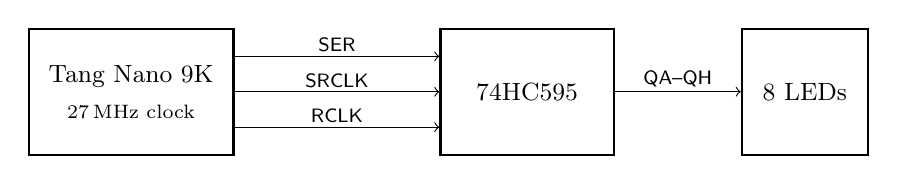
\begin{tikzpicture}[box/.style={draw, thick, minimum height=1.6cm, align=center, font=\small},
      wire/.style={->}, lbl/.style={font=\scriptsize\sffamily, above, inner sep=1.5pt}]
    \node[box, minimum width=2.6cm] (fpga) {\name{Tang Nano 9K}\\[0.2em]\scriptsize 27\,MHz clock};
    \node[box, minimum width=2.2cm, right=2.6cm of fpga] (sr) {\name{74HC595}};
    \node[box, minimum width=1.6cm, right=1.6cm of sr] (leds) {8 LEDs};
    \draw[wire] ([yshift=0.45cm]fpga.east) -- node[lbl] {SER} ([yshift=0.45cm]sr.west);
    \draw[wire] (fpga.east) -- node[lbl] {SRCLK} (sr.west);
    \draw[wire] ([yshift=-0.45cm]fpga.east) -- node[lbl] {RCLK} ([yshift=-0.45cm]sr.west);
    \draw[wire] (sr.east) -- node[lbl] {QA--QH} (leds.west);
  \end{tikzpicture}
\end{figure}

The breadboard holds a \name{74HC595}, with eight LEDs on its outputs and three buttons on its inputs \name{SER}, \name{SRCLK}, and \name{RCLK}. Here the FPGA takes the place of the buttons. Once per half-second tick, it does what the buttons do, in two ways:
\begin{itemize}[nosep]
  \item \textbf{Forward, a bit at a time.} On the first tick, the FPGA puts a 1 into the shift register, and on each of the next seven ticks, it puts in a 0. Every tick shifts and latches, so the lit LED walks from \name{QA} to \name{QH}.
  \item \textbf{Backward, a byte at a time.} Shifting moves a bit only towards \name{QH}. To walk from \name{QH} to \name{QA}, each tick therefore writes all eight bits, with the 1 one place further back, and then latches them.
\end{itemize}

\section*{The FPGA’s pins}

\begin{figure}[H]
  \centering
  \begin{minipage}[c]{0.72\linewidth}
  \centering
  \resizebox{\linewidth}{!}{%
  \begin{tikzpicture}[
      port/.style={font=\footnotesize\ttfamily},
      pin/.style={font=\scriptsize, above, inner sep=1.5pt},
      blk/.style={draw, thick, align=center, font=\small, minimum height=0.9cm},
      hdr/.style={draw, fill=white, circle, inner sep=1.6pt},
      title/.style={font=\small\bfseries, inner sep=3pt}]
    % the development board, and the FPGA on it
    \draw[black!45, rounded corners=3pt] (-3.6,-2.9) rectangle (3.4,1.9);
    \node[title, anchor=south west] at (-3.6,-2.9) {\name{Tang Nano 9K}};
    \draw[thick] (-1.8,-1.3) rectangle (1.8,1.4);
    \node[title, anchor=north] at (0,1.4) {\name{GW1NR-9}};
    \node[port, anchor=west] at (-1.75,-0.3) {sys\_clk};
    \node[port, anchor=east] at (1.75,0.3) {ser};
    \node[port, anchor=east] at (1.75,-0.3) {srclk};
    \node[port, anchor=east] at (1.75,-0.9) {rclk};
    \pic at (-2.9,-0.3) {crystal};
    \node[font=\scriptsize, below] at (-2.9,-0.7) {27\,MHz};
    \draw[->] (-2.6,-0.3) -- (-1.8,-0.3);
    \node[pin] at (-2.1,-0.3) {52};
    % FPGA pins, header pins, and the 595's pins
    \draw[thick] (5.8,-1.4) rectangle (7.8,0.9);
    \node[font=\small] at (6.8,1.15) {\name{74HC595}};
    \foreach \y/\f/\h/\c/\n in {0.3/25/L5/14/SER, -0.3/26/L6/11/SRCLK, -0.9/27/L7/12/RCLK} {
      \draw[->] (1.8,\y) -- (5.8,\y);
      \node[pin] at (2.1,\y) {\f};
      \node[hdr] at (3.4,\y) {};
      \node[pin, anchor=south west] at (3.5,\y) {\name{\h}};
      \node[pin] at (5.5,\y) {\c};
      \node[font=\footnotesize, anchor=west] at (5.85,\y) {\name{\n}};
    }
    % the breadboard's rails
    \foreach \y/\h/\r in {-1.9/R24/{$+$ rail, 3.3\,V}, -2.5/R23/{$-$ rail, \name{GND}}} {
      \draw (3.4,\y) -- (5.6,\y);
      \node[anchor=west, font=\small, inner sep=0pt] at (5.8,\y) {\r};
      \node[hdr] at (3.4,\y) {};
      \node[pin, anchor=south west] at (3.5,\y) {\name{\h}};
    }
  \end{tikzpicture}}
  \end{minipage}\hfill
  \begin{minipage}[c]{0.26\linewidth}
  \centering
  \boardpins{l/5/L5/-1, l/6/L6/0, l/7/L7/1, r/23/R23/-0.5, r/24/R24/0.5}
  \end{minipage}
  \caption{Left: the \name{GW1NR-9} is the board’s FPGA chip. Inside its box are the design’s port names, and on its edge are the chip’s pin numbers, which the \name{.cst} file uses. On the board’s edge are the header pins that the wires plug into. Next to the \name{595} are its own pin numbers. Right: the same header pins on the board, seen from above with the USB-C connector at the top~\cite{topview}. L and R are the left-hand and right-hand rows. Their pins are counted from the USB-C end, where pin 1 of each row has a square pad. \name{R24} is \name{3V3}, and \name{R23} is \name{GND}~\cite[p.~2]{schematic}.}
\end{figure}

\name{SER} is the serial input, which carries the next bit. \name{SRCLK} is the shift-register clock, and on its rising edge the shift register shifts. \name{RCLK} is the register clock, and on its rising edge the outputs copy the shift register.

The \name{595} runs at 3.3\,V, so it needs 3.3\,V pins, and not every FPGA pin is one. The pins of the onboard LEDs and buttons run at 1.8\,V, and a 1.8\,V high is too low for the \name{595} to read as \name{HIGH}. In the board’s schematic~\cite{schematic}, pins whose names end in \name{\_1V8} are 1.8\,V pins. Pins 25 to 30 are 3.3\,V pins, and nothing else on the board is wired to them. This design uses 25, 26, and 27.

\section*{Rewiring}

The buttons, their pull-downs, and the \name{SRCLK} capacitor stay where they are.
\begin{enumerate}
  \item \textbf{Three jumpers move.} Three jumpers run from the \name{595}’s \name{SER}, \name{SRCLK}, and \name{RCLK} to the button nodes. Each one comes off at its button end and goes to an FPGA pin: 25, 26, and 27, in that order. The button circuits stay on the breadboard, joined to nothing.
  \item \textbf{Power from the \name{Tang Nano}.} The power module comes out. The board’s \name{3V3} pin goes to the $+$ rail, and a \name{GND} pin goes to the $-$ rail, so the board and the breadboard share one supply and one ground.
\end{enumerate}

With the jumpers off the button nodes, the \name{595}’s three inputs have no pull-down. While the FPGA loads its design, they float and may shift in a few stray bits. The forward walk pushes them out within its first eight ticks, and the backward walk overwrites them on its first tick.

\textbf{Is there enough current?} Eight LEDs at about 4\,mA each draw 32\,mA from the 3.3\,V rail. That rail comes from one channel of the board’s \name{TMI7003C}, a step-down converter with three channels that supply up to 1.5\,A each~\cite{tmi7003c}~\cite[p.~3]{schematic}. Upstream, the board takes 5\,V from the Mac’s USB-C port. Its 5.1\,kΩ resistors on \name{CC1} and \name{CC2}~\cite[p.~4]{schematic} make the Mac treat it as a powered device, which gets at least 500\,mA. The LEDs’ 0.1\,W adds about 25\,mA at 5\,V.

\section*{Timing}

The \name{595} needs time between the steps you pressed by hand. Its datasheet~\cite[§6.6, p.~6]{sn74hc595} gives the minimum times at three supply voltages:

\begin{center}
\begin{tabular}{r>{\raggedright\arraybackslash}p{7.4cm}rrr}
  \toprule
  & & \multicolumn{3}{c}{Minimum (ns) at} \\
  \cmidrule(l){3-5}
  & Requirement & 2\,V & 4.5\,V & 6\,V \\
  \midrule
  1 & serial input (\name{SER}) steady before the shift-register clock (\name{SRCLK}) rises & 125 & 25 & 21 \\
  2 & shift-register clock (\name{SRCLK}) rises before the register clock (\name{RCLK}) rises & 94 & 19 & 16 \\
  3 & \name{SRCLK} or \name{RCLK} high, or low & 100 & 20 & 17 \\
  \bottomrule
\end{tabular}
\end{center}

Reading across a row shows that the same step needs five times longer at 2\,V than at 4.5\,V. The lower the supply, the slower the chip. The table has no 3.3\,V column. Since 3.3\,V lies between 2 and 4.5\,V, its minimums lie between those two columns, and the 2\,V figures, which are the larger ones, are always enough. These figures are for the \name{SN74HC595}, from −40 to 85\,°C.

\section*{The same times in clock cycles}

The FPGA measures time by counting cycles of the board’s 27\,MHz clock, which is called the system clock, \texttt{sys\_clk} in the constraint files. One cycle is 37\,ns. Rounded up to whole cycles, the three minimums are:

\begin{center}
\begin{tabular}{rlrr}
  \toprule
  & Requirement & Minimum (ns) & Minimum (cycles) \\
  \midrule
  1 & \name{SER} steady before \name{SRCLK} rises & 125 & 4 \\
  2 & \name{SRCLK} rises before \name{RCLK} rises & 94 & 3 \\
  3 & \name{SRCLK} or \name{RCLK} high, or low & 100 & 3 \\
  \bottomrule
\end{tabular}
\end{center}

The name \texttt{sys\_clk} is a convention. A Verilog module’s clock input is usually called \texttt{clk}, whichever clock drives it. The board’s clock pin, from which every other clock comes, is called \texttt{sys\_clk}. In larger designs, modules sit inside a top level, and the top level wires \texttt{sys\_clk}, or a faster clock made from it, into each module’s \texttt{clk}. Each walk is a single module, so its clock input is the pin itself, \texttt{sys\_clk}.

From here on, the design counts in cycles. It spaces its steps 27 cycles apart, which is 1\,µs. That is a round number on the analyser, and more than six times the longest minimum. One forward tick sets \name{SER}, shifts, and latches, and it takes 81 cycles, or 3\,µs. The LEDs then hold still for the rest of the half second.

\begin{figure}[H]
  \centering
  \begin{tikztimingtable}[timing/slope=0.1, xscale=1.2, yscale=1.4, timing/rowdist=3, timing/name/.style={font=\small\sffamily}]
    SER   & L 11H \\
    SRCLK & 4L 3H 5L \\
    RCLK  & 7L 3H 2L \\
  \extracode
    \vertlines[black!20]{1.05,4.05,7.05,10.05}  % through each edge's midpoint: the slope is 0.1
    \foreach \x/\c in {1.05/0, 4.05/27, 7.05/54, 10.05/81} \node[font=\scriptsize, below] at (\x,-6.3) {\c};
    \node[font=\scriptsize, anchor=west] at (12.2,-6.55) {cycles};
    \draw[decorate, decoration={brace, amplitude=4pt}] (1.05,1.25) -- node[above=4pt, font=\scriptsize] {27 $\geq$ 4 (row 1)} (4.05,1.25);
    \draw[decorate, decoration={brace, amplitude=4pt}] (4.05,-1.75) -- node[above=4pt, font=\scriptsize] {27 $\geq$ 3 (rows 2, 3)} (7.05,-1.75);
    \draw[decorate, decoration={brace, amplitude=4pt}] (7.05,-4.75) -- node[above=4pt, font=\scriptsize] {27 $\geq$ 3 (row 3)} (10.05,-4.75);
  \end{tikztimingtable}
  \caption{One forward tick that sends in a 1, counted in cycles of the 27\,MHz clock. Each brace shows a time that the design gives, next to the minimum that the \name{595} needs.}
\end{figure}

\section*{Register-transfer level design: forward}

The design is in \name{rtl/walk/walk.v}. It is described here one block at a time, in the order of the file.

\subsection*{Ports}

\inputminted[firstline=4, lastline=9]{verilog}{../rtl/walk/walk.v}

The module has one input, the 27\,MHz clock, and three outputs, one for each input of the \name{595}. Each output is declared as \texttt{reg} because an \texttt{always} block assigns it, and each starts at 0, the value written after it. The block is clocked, so each output becomes a flip-flop that drives its pin.

\subsection*{Constants}

\inputminted[firstline=11, lastline=12]{verilog}{../rtl/walk/walk.v}

\texttt{TICK} is the length of one tick in clock cycles: 13\,500\,000 cycles of 37\,ns make half a second. It is a \texttt{parameter}, so the testbench can change it from outside the module and shorten the tick. \texttt{STEP} is the gap between two steps, 27 cycles, which is 1\,µs. It is a \texttt{localparam}, which can’t be changed from outside.

\subsection*{Counters}

\inputminted[firstline=14, lastline=15]{verilog}{../rtl/walk/walk.v}

\texttt{t} counts the cycles of the current tick, from 0 to \texttt{TICK - 1}. It needs 24 bits, because 13\,499\,999 is less than $2^{24}$, which is 16\,777\,216. \texttt{k} counts the ticks from 0 to 7, in 3 bits. The 1 goes into the shift register on tick 0, and a 0 goes in on each of the other seven ticks.

\subsection*{The tick}

\inputminted[firstline=17, lastline=25]{verilog}{../rtl/walk/walk.v}

This block runs at every rising edge of \texttt{sys\_clk}. The operator \texttt{<=} is the \emph{nonblocking} assignment, which is the one used for registers. With it, every register in the block takes its new value at the same clock edge, computed from the values that the registers had before that edge.

The first line advances \texttt{t}. The expression \texttt{a ? b : c} is \texttt{b} when \texttt{a} is true, and \texttt{c} otherwise. So \texttt{t} goes back to 0 on the last cycle of the tick, and it counts up by one on every other cycle.

The \texttt{case} statement compares \texttt{t} with each label and runs the line whose label matches. On every other cycle, nothing in the \texttt{case} runs, and the three outputs keep their values.

\begin{itemize}
  \item At cycle 0, \texttt{ser} takes the value of \texttt{k == 0}. It is 1 on tick 0, and 0 on the other seven ticks.
  \item At cycle \texttt{STEP}, \texttt{srclk} rises, and the \name{595} shifts \name{SER} in.
  \item At cycle \texttt{2 * STEP}, \texttt{srclk} falls and \texttt{rclk} rises, and the \name{595} copies the shift register onto its outputs.
  \item At cycle \texttt{3 * STEP}, \texttt{rclk} falls, and \texttt{k} moves on to the next tick.
\end{itemize}

The order is the same as with the buttons: \name{SER} first, then \name{SRCLK}, then \name{RCLK}. \texttt{k} is 3 bits wide, so it counts to 7 and wraps to 0 on its own. Every eighth tick therefore sends in a new 1, just as the old one leaves \name{QH}.

\name{rtl/walk/walk.cst} puts \texttt{sys\_clk} on pin 52, and \texttt{ser}, \texttt{srclk}, and \texttt{rclk} on pins 25, 26, and 27, all as \texttt{LVCMOS33}. \texttt{make flash walk} builds the design and writes it to the board’s flash. \texttt{make rtl walk} draws its RTL, which has a counter, three comparators, and four registers.

\section*{Register-transfer level design: backward}

The design is in \name{rtl/walkback/walkback.v}. Its ports and constants are the same as in the forward walk, so the description starts with its counters.

\subsection*{Counters}

\inputminted[firstline=14, lastline=17]{verilog}{../rtl/walkback/walkback.v}

\texttt{t} counts the cycles of the tick, as in the forward walk. \texttt{c} counts the cycles of the current step, from 0 to \texttt{STEP - 1}, which is 26, so it needs 5 bits. \texttt{n} numbers the steps of the tick. Steps 0 to 15 shift the eight bits in, steps 16 and 17 latch them, and at step 18 the design waits until the tick ends. \texttt{p} is the place of the lit LED, from 7, which is \name{QH}, down to 0, which is \name{QA}. It starts at 7, so the walk starts at \name{QH}.

\subsection*{Counting the steps}

\inputminted[firstline=19, lastline=25]{verilog}{../rtl/walkback/walkback.v}

\texttt{t} goes back to 0 at the end of each tick, as before, and \texttt{c} goes back to 0 at the end of each step. \texttt{n} goes back to 0 on the last cycle of the tick. Otherwise, \texttt{n} moves on to the next step on the last cycle of each step, until it reaches 18. There it stops and waits for the next tick.

\subsection*{What each step does}

\inputminted[firstline=27, lastline=38]{verilog}{../rtl/walkback/walkback.v}

The actions happen only on the first cycle of each step, when \texttt{c} is 0, so they are \texttt{STEP} cycles apart.

\begin{itemize}
  \item Steps 0 to 15 send the eight bits in pairs. On an even step, \texttt{n[0]}, the lowest bit of \texttt{n}, is 0. That step drops \texttt{srclk} and sets \texttt{ser}. On the odd step after it, \texttt{srclk} rises, and the \name{595} shifts \name{SER} in.
  \item \texttt{n[3:1]} is bits 3 to 1 of \texttt{n}, which is the number of the pair, from 0 to 7. The first bit in ends at \name{QH}, so the bit sent on pair \texttt{n[3:1]} lands on output $7 - \texttt{n[3:1]}$. \texttt{ser} is 1 only for the bit that lands on \texttt{p}.
  \item Step 16 drops \texttt{srclk} and raises \texttt{rclk}, so the \name{595} copies the shift register onto its outputs. Step 17 drops \texttt{rclk} and moves \texttt{p} one place back. \texttt{p} is 3 bits wide, so from 0 it wraps to 7.
  \item The \texttt{default} branch covers every other step, and \texttt{if (n < 16)} keeps steps 18 and above from doing anything.
\end{itemize}

Every gap is still 27 cycles, so the timing figure holds for each pair. A tick takes 18\,µs.

\name{rtl/walkback/walkback.cst} uses the same pins. \texttt{make flash walkback} builds the design and writes it to the board’s flash.

\section*{In simulation}

Before the board, both designs run in a simulator, \name{Icarus Verilog}, which is part of the open flow. A testbench, \name{sim/walk\_tb.v}, feeds each design a 27\,MHz clock and connects it to a model of the \name{595}. The model has a shift register, which takes \name{SER} on the rising edge of \name{SRCLK}, and an output register, which copies the shift register on the rising edge of \name{RCLK}. After every tick, the testbench prints the eight LEDs, with \name{QA} on the left and \texttt{*} for a lit one. A tick is shortened to 1000 cycles, because half a second is 13.5 million cycles.

\begin{minted}{bash}
iverilog -g2012 -o build/walk_tb sim/walk_tb.v rtl/walk/walk.v rtl/walkback/walkback.v
vvp -n build/walk_tb
\end{minted}

\inputminted{text}{data/walk_tb.txt}

Both models start from a made-up power-up pattern. In the forward walk, the old pattern shifts out towards \name{QH} while 0s come in behind it. From tick 7 on, one LED is lit, and the walk restarts at \name{QA} on tick 8. In the backward walk, the first tick overwrites all eight outputs at once, so one LED is lit from the start, and it walks from \name{QH} to \name{QA}. The last four lines give, in cycles, the shortest of each of the three gaps in the timing table, measured on every edge. None is below its minimum. \hyperref[app:testbench]{The appendix} explains how the testbench works and shows its code.

\section*{On the analyser}

The analyser’s \name{CH0} goes on \name{SER}, \name{CH1} on \name{SRCLK}, \name{CH2} on \name{RCLK}, and its \name{GND} to \name{GND}. Trigger on the rising edge of \name{CH1}, at 4\,MS/s or more. In the forward walk, each tick shows the same three edges, 1\,µs apart, and \name{SER} is high on one tick in eight. \name{QH'} (pin 9) carries the bit that leaves the register. With \name{CH3} on it, the analyser shows the 1 coming out eight ticks after it went in. In the backward walk, each tick shows eight \name{SRCLK} pulses and one \name{RCLK} pulse, with \name{SER} high during one of them.

\section*{Done when}

In the forward walk, one lit LED walks from \name{QA} to \name{QH}, one step every half second, and starts again at \name{QA}. After the first eight ticks, exactly one LED is lit at all times. In the backward walk, the lit LED walks from \name{QH} to \name{QA}, and exactly one LED is lit from the first tick.

\appendix
\section{The testbench}\label{app:testbench}

This appendix goes through \name{sim/walk\_tb.v} part by part. A testbench is Verilog that never goes on the chip. It has no ports, makes its own clock, and prints what it sees. \texttt{\#18.5} waits 18.5\,ns of simulated time, in the unit that \texttt{`timescale} sets. Delays and \texttt{\$display} exist only in the simulator.

\subsection*{Clock and the two designs}

\inputminted[firstline=7, lastline=20]{verilog}{../sim/walk_tb.v}

The clock flips every 18.5\,ns, so a full cycle takes 37\,ns, which is 27\,MHz. Each design is placed with \texttt{\#(.TICK(TICK))}, which replaces its \texttt{TICK} parameter, so a tick lasts 1000 cycles instead of 13.5 million. Nothing else in the designs changes.

\subsection*{The \name{595} model}

\inputminted[firstline=22, lastline=29]{verilog}{../sim/walk_tb.v}

Each walk gets its own chip. \texttt{f\_shift} is the shift register. On the rising edge of \name{SRCLK}, every bit moves one place towards \name{QH}, and \name{SER} comes in at \name{QA}, bit 0. \texttt{f\_q} is the output register, which holds the eight LEDs. On the rising edge of \name{RCLK}, it copies the shift register. This model behaves like the chip at flip-flop level, without its timing.

\subsection*{The gaps}

\inputminted[firstline=62, lastline=85]{verilog}{../sim/walk_tb.v}

The model accepts any timing, so the testbench checks the timing separately. \texttt{cycle} counts clock cycles from the start. Each line remembers the cycle of its last change. At each edge that the datasheet limits, the testbench compares the current cycle with that one and keeps the shortest gap seen. There are three such gaps: from a change of \name{SER} to the rising edge of \name{SRCLK} (row 1), from the rising edge of \name{SRCLK} to the rising edge of \name{RCLK} (row 2), and between two changes of \name{SRCLK} or of \name{RCLK}, which is how long the line stays high or low (row 3). The first change of each line, from unknown to 0 at time 0, is not a pulse, and the testbench skips it.

\subsection*{Printing}

\inputminted[firstline=37, lastline=58]{verilog}{../sim/walk_tb.v}

\texttt{leds} turns the eight outputs into eight characters, \name{QA} first. The \texttt{initial} block prints the power-up state. Then it waits one tick at a time and prints both walks side by side. After sixteen ticks, which are two full walks, it prints the shortest gaps and stops.

\begin{thebibliography}{SN74}
\bibitem[SN74]{sn74hc595} Texas Instruments, \textit{SNx4HC595 8-Bit Shift Registers With 3-State Output Registers}, SCLS041J, Oct 2021, \url{https://www.ti.com/lit/ds/symlink/sn74hc595.pdf}.
\bibitem[TMI]{tmi7003c} Toll Semiconductor, \textit{TMI7003C: 3 Channels 1.5A, 1.5MHz DC/DC Step-Down PMU}, V1.5, Jul 2024.
\bibitem[TN9K]{schematic} Sipeed, \textit{Tang Nano 9K schematic}, \name{Tang\_Nano\_9k\_3672\_Schematic.pdf}, \url{https://dl.sipeed.com/shareURL/TANG/Nano%209K/2_Schematic}.
\bibitem[Top]{topview} Sipeed, \textit{Tang Nano 9K top designator drawing}, \name{Tang\_Nano\_9K\_3672\_Top\_Designator\_Drawing.pdf}, \url{https://dl.sipeed.com/shareURL/TANG/Nano\%209K}; in the repo as \name{docs/assets/tang-nano-9k-top.pdf}.
\end{thebibliography}

\end{document}
